\chapter{Исследовательская часть}

В данном разделе будут приведены примеры работы программ и сравнительный анализ алгоритмов на основе полученных данных.

\section{Технические характеристики}

Технические характеристики устройства, на котором выполнялось исследование:

\begin{itemize}
	\item операционная система:Windows 11 Home Single Language 23H2;
	\item память: 16 Гб;
	\item процессор: 1,8 ГГц 4-ядерный процессор Intel Core i7.
\end{itemize}

Во время тестирования устройство было подключено к сети электропитания, нагружено приложениями окружения и самой системой тестирования.

\section{Время выполнения реализаций алгоритмов}

Замеры процессорного времени выполнения реализаций алгоритмов произведены при помощи функции clock() из библиотеки time языка C. Данная функция возвращает возвращает количество временных тактов, прошедших с начала запуска программы.

Замеры проводились для строк одинаковой длины от 0 до 12 символов по 1000 раз (Рисунок~\ref{fig:graph-l}) до 1000 символов (Рисунок~\ref{fig:graph-lnr-lrc}).

\begin{figure}[H]
	\centering
	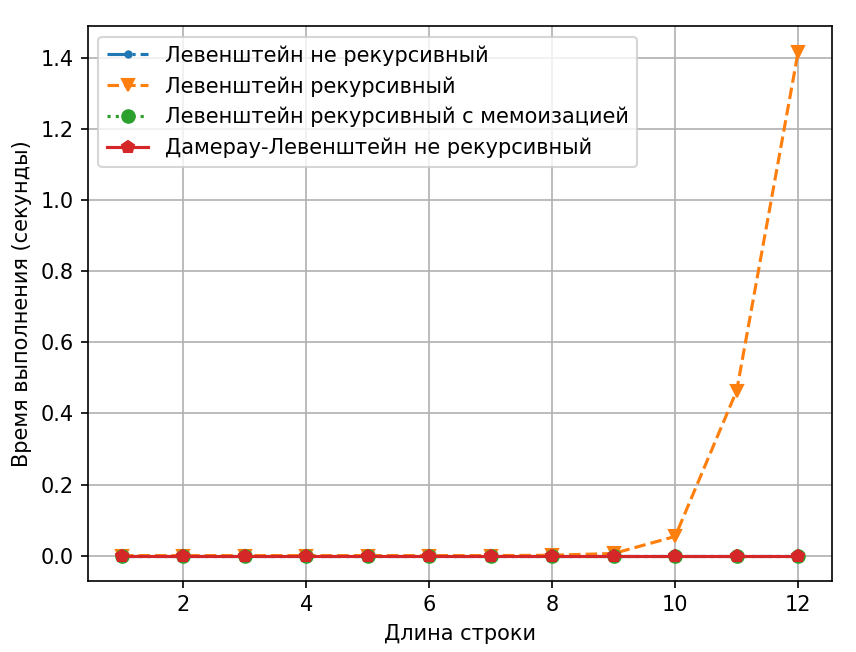
\includegraphics[height=0.4\textheight, page=1]{inc/img/short_len.png}
	\caption{Сравнение по времени выполнения реализаций алгоритмов нахождения расстояния Левенштейна}
	\label{fig:graph-l}
\end{figure}

\begin{figure}[H]
	\centering
	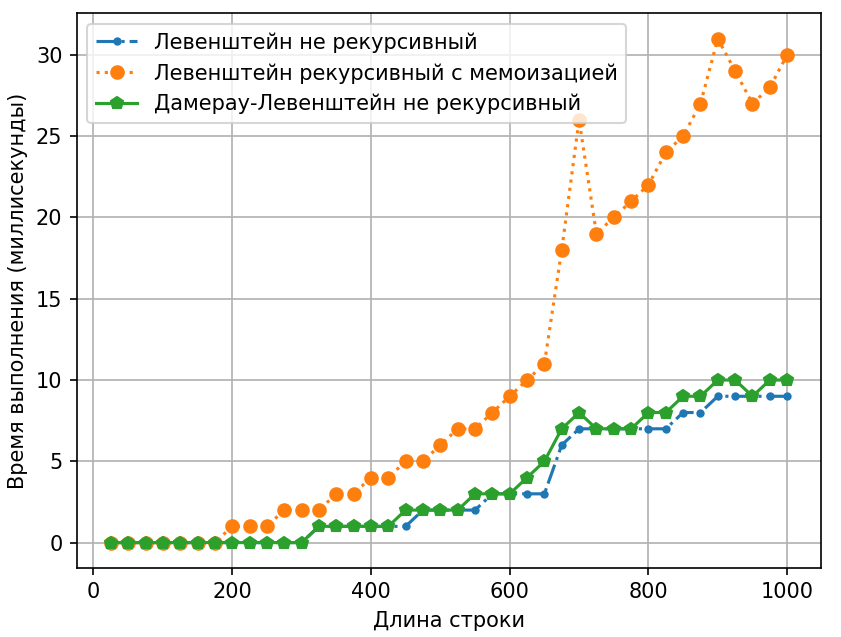
\includegraphics[height=0.4\textheight, page=1]{inc/img/long_len.png}
	\caption{Сравнение по времени выполнения нерекурсивной и рекурсивной с кэшем реализаций алгоритмов нахождения расстояния Левенштейна с не рекурсивной реализацией алгоритма Дамерау~---~Левенштейна}
	\label{fig:graph-lnr-lrc}
\end{figure}

\section*{Вывод}

Исходя из замеров по времени, рекурсивная реализация алгоритма нахождения расстояния Левенштейна работает дольше остальных. Наименее затратным по времени оказалась не рекурсивная реализация алгоритма нахождения расстояния Левенштейна.

Исходя из замеров по памяти, не рекурсивные и рекурсивные с кэшем реализации алгоритмов проигрывают рекурсивным.